\section{Primario non sferico}

\begin{frame}{Sviluppo in multipoli energia potenziale}

\begin{align*}
V(\vec{r})=-\frac{Gm}{r}[\int\rho'\,d^3r'+\cos{\theta}\int\frac{r'}{r}\cos{\theta'}\rho(\vec{r}')\,d^3r'\\
+\frac{1}{2}(3\cos{\theta}^2-1)\int\frac{r'}{r}\frac{1}{2}(3\cos{\theta}^2-1)\rho(\vec{r}')\,d^3r'+\ldots]
\end{align*}

\begin{block}{Potenziale di quadrupolo}

\begin{equation*}
V(\vec{r})=-\frac{Gm}{r}[M+\frac{1}{2r^2}(A-C)(3\cos{\theta}^2-1)+\ldots]
\end{equation*}

\end{block}

\end{frame}

\begin{wordonframe}{Momento inerzia e $J_2$}

\begin{align*}
&I_x=I_y=A=\int(x'^2+z'^2)\rho\,d^3r'=\int(y'^2+z'^2)\rho\,d^3r'\\
&I_z=C=\int(x'^2+y'^2)\rho\,d^3r'\\
&J_2=\frac{C-A}{MR^2}\, GmM=k^2\mu\\
\end{align*}

$J_2>0$ for any planet flatten by rotation

\begin{block}{Terra-Luna}

\begin{align*}
J_2^{\oplus}\approx\num{e-3}\\
(\frac{R}{r})^2\approx(\frac{1}{60})^2\approx\num{3e-4}\\
\frac{V_Q}{V_N}\approx\num{3e-7}
\end{align*}

\end{block}

\end{wordonframe}

\begin{frame}{Forza perturbatrice}

\begin{columns}
\begin{column}{0.6\textwidth}

\begin{align*}
&V=-\frac{k^2\mu}{r}+V'\\
&V'=-\frac{3Q}{r^5}(\frac{1}{3}-\cos{\theta}^2)\\
&Q=\frac{1}{2}k^2\mu R^2J_2
\end{align*}

\end{column}
\begin{column}{0.4\textwidth}

\begin{figure}[!ht]
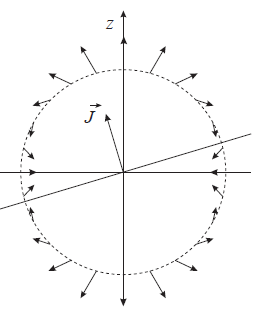
\includegraphics[width=\textwidth]{perturbation}
\end{figure}

\end{column}
\end{columns}

$e$, $i$, $|\vec{J}|$ non variano in media su un periodo.

\begin{block}{Periodo del moto radiale (i=0)}

Traiettoria a ''rosetta'':

\begin{equation*}
T_{\lambda}=\frac{\pi}{\Delta}T_{r}
\end{equation*}

\end{block}

\end{frame}

\begin{wordonframe}{forza perturbatrice}

\begin{align*}
&f_x=3Qr\expy{-4}(5\cos{\theta}^2-1)\sin{\theta}\cos{\lambda}\\
&f_y=3Qr\expy{-4}(5\cos{\theta}^2-1)\sin{\theta}\sin{\lambda}\\
&f_z=3Qr\expy{-4}(5\cos{\theta}^2-1)\cos{\theta}
\end{align*}

\begin{block}{Integrali primi del moto ($i=0$)}
\begin{align*}
&\mu r^2\dot{\lambda}^2=J\\
&\frac{1}{2}\mu\dot{r}^2-\frac{k^2\mu}{r}+\frac{J^2}{2\mu r^2}+V'=E
\end{align*}
\end{block}

\begin{align*}
&T_r=2\int_{r_{min}}^{r_{max}}\,dr(\frac{2E}{\mu}-\frac{2V'}{\mu}-\frac{J^2}{\mu^2r^2}+\frac{2k^2}{r})\expy{-\frac{1}{2}}\\
&\Delta=\frac{J}{\mu}\int_{r_{min}}^{r_{max}}\,dr(\frac{2E}{\mu}-\frac{2V'}{\mu}-\frac{J^2}{\mu^2r^2}+\frac{2k^2}{r})\expy{-\frac{1}{2}}
\end{align*}

\end{wordonframe}

\begin{frame}{Effetti su orbita}

\begin{itemize}
\item Linea dei nodi regresses for prograde orbit ($i\neq\pi/2$) - Piano orbita ruota backward

\item $\forall i<\ang{46.5}$ il pericentro ruota in avanti.

\item $\forall i<\sin{\sqrt{\frac{2}{3}}}\expy{-1}=\ang{54.7}$ mean anomaly increases at rate greater than n: orbital period is less then for keplerian orbit about spherical planet of same mass.

\item We can determine $J_2$ for planets having satellites in eccentric/inclined orbit.

\end{itemize}

\end{frame}

\section{Metodo di Newton}


\begin{equation*}
\mu\ddot{r}=f+\frac{c}{r^3}+\frac{J^2}{\mu r^3}=f+\frac{J'^2}{\mu r^3}
\end{equation*}


Stessa moto radiale con diverso j; moto angolare perturbato ha velocit\'a proporzionale a quello imperturbato: $\frac{\dot{\lambda}}{\dot{\lambda'}}=\frac{J}{J'}$.

\begin{block}{Orbita quasi-circolare}
Moto medio del pericentro: $\frac{3}{2}n\frac{R^2}{a^2}J_2$.
\end{block}

\begin{wordonframe}{Perturbazione orbita quasi-circolare}

f forza centrale

\begin{align*}
V'(\theta=\pi/2)=-\frac{3Q}{r^4}\approx\frac{3Q}{r^2a^2}-\frac{6Q}{ar^3}+o((r-a)^2)
\end{align*}

\end{wordonframe}

\section{Precessione luni-solare}

\begin{frame}{Momento rispetto al CM della Terra}

\begin{columns}  \begin{column}{0.3\textwidth}

\begin{figure}[!ht]

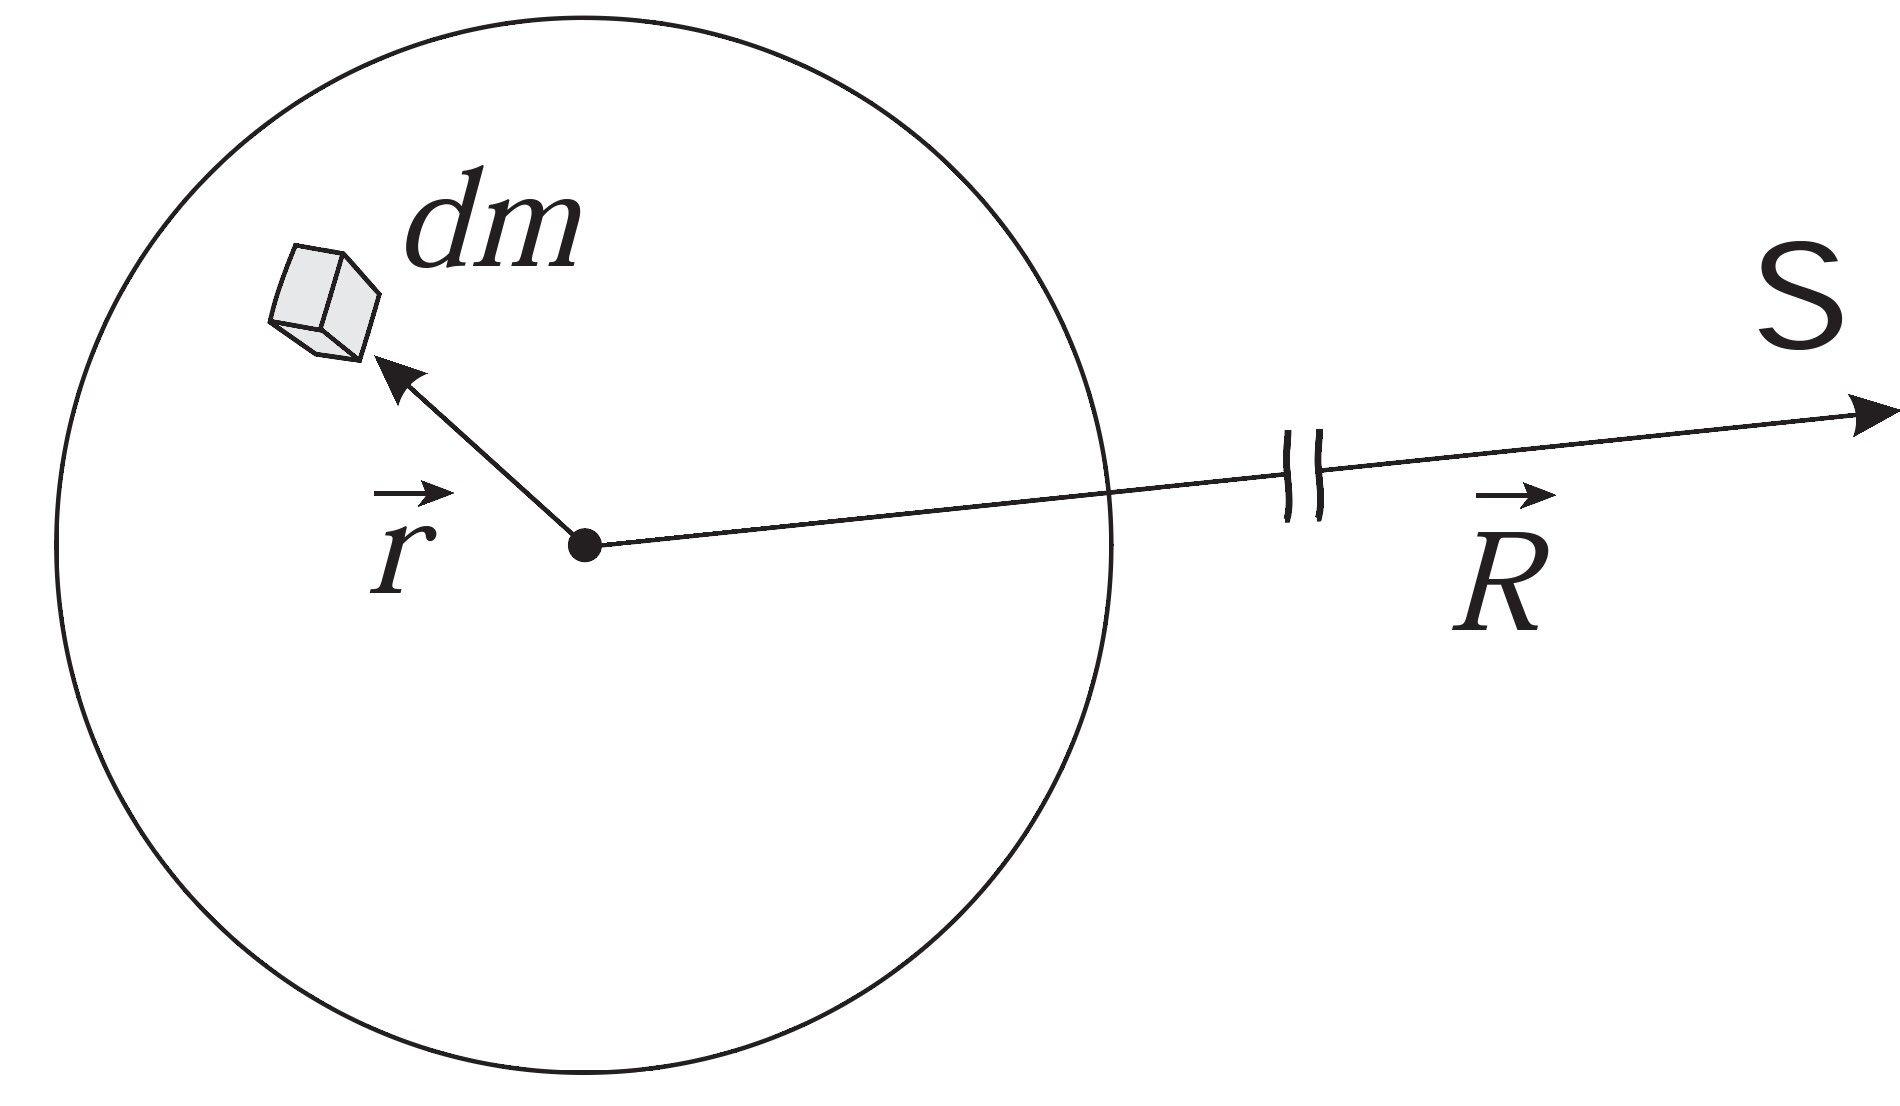
\includegraphics[width=\textwidth]{Sunearth}

\end{figure}

\end{column} \begin{column}{0.7\textwidth}

\begin{equation*}
d\vec{K}=\vec{r}\wedge d\vec{F}=\frac{GM\,dm}{R^3}(1+3\frac{\scap{R}{r}}{R^2})\vecp{r}{R}
\end{equation*}

\end{column}  \end{columns}

\begin{block}{Media annua}

\begin{columns}  \begin{column}{0.4\textwidth}

\begin{align*}
&\bar{K}_{\xi}=\frac{3GM}{2R^3}(C-A)\sin{\epsilon}\cos{\epsilon}\\
&\bar{K}_{\eta}=\bar{K}_{\zeta}=0
\end{align*}

\end{column} \begin{column}{0.6\textwidth}

\begin{figure}[!ht]

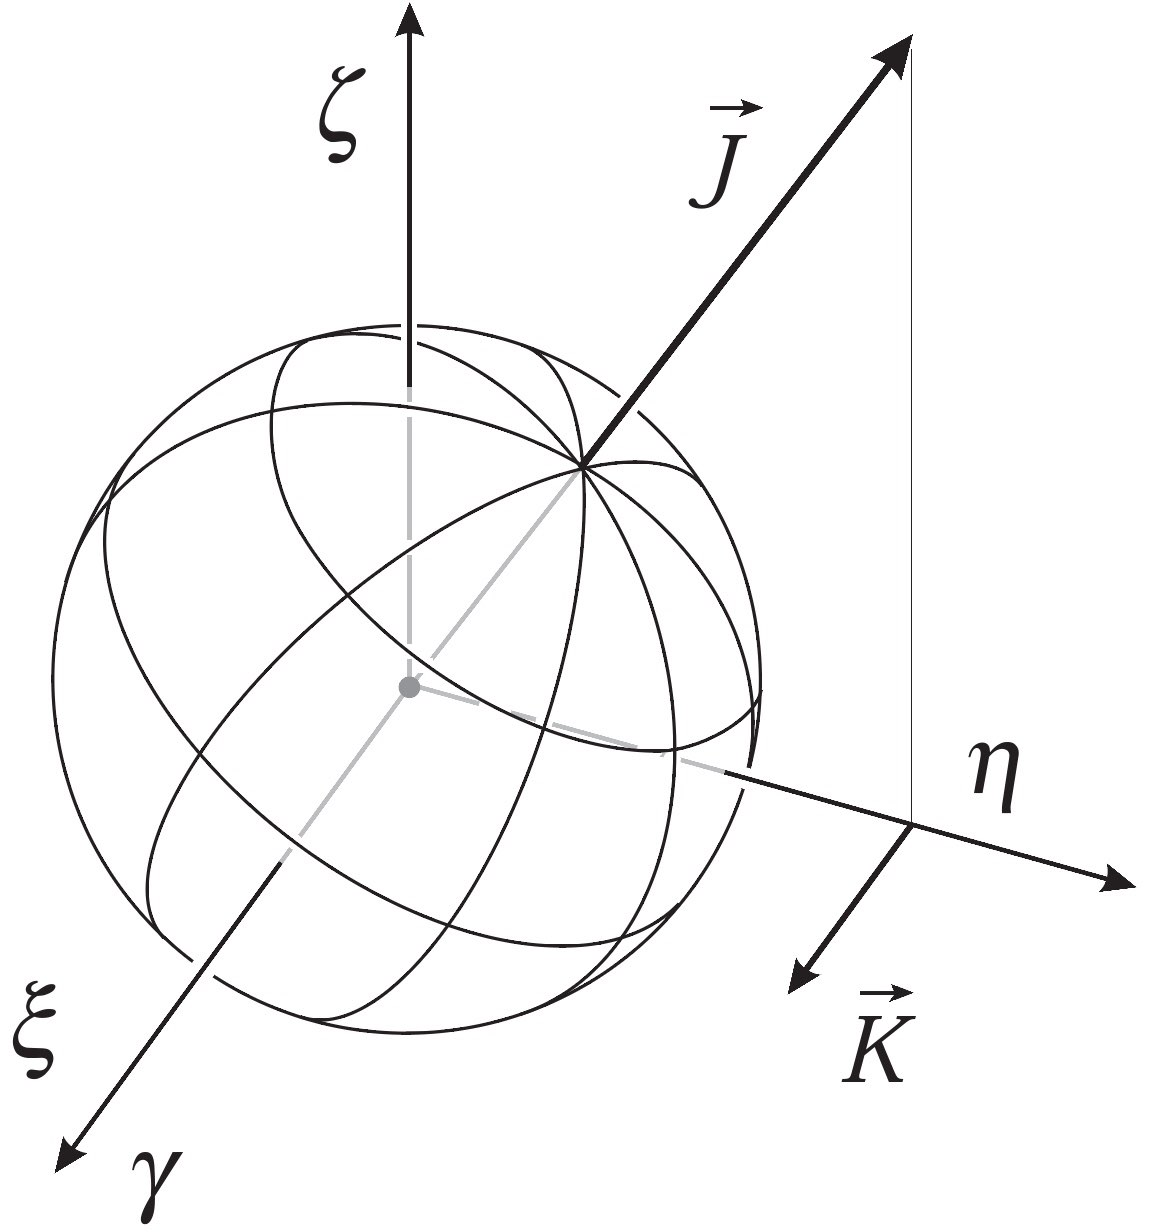
\includegraphics[width=\textwidth]{eclcoord}

\end{figure}

\end{column}
\end{columns}

\end{block}

\begin{block}{Velocit\'a di precessione della Terra dovuta all'attrazione lunisolare}

\begin{equation*}
P=P_{\odot}+P_{\leftmoon}\approx\ang{;;50.3}\si{\per\year}
\end{equation*}


\end{block}


\end{frame}

\begin{wordonframe}{Momento delle forze}

\begin{align*}
&K_x=\frac{3GM}{2R^5}(C-A)YZ\\
&K_y=\frac{3GM}{2R^5}(C-A)XZ\\
&K_z=0
\end{align*}

Coordinate eclittiche: $\lambda$ longitudine eclittica del SOle, $\epsilon$ obliquit\'a dell'eclittica

\end{wordonframe}


\section{Perturbazioni}

\begin{frame}{Meccanica analitica}

\begin{columns}  \begin{column}{0.5\textwidth}

\begin{block}{Approssimazione di quadrupolo}

\begin{align*}
&H=H_0+H_1\\
&H_0=-\frac{k^4\mu^3}{2J_{\phi}^2}\\
&H_1=\frac{3}{2}R^2J_2k^2\mu\frac{1}{r^3}(\sin^2{\beta}-\frac{1}{3})
\end{align*}


\end{block}

\end{column}

\begin{column}{0.5\textwidth}

\begin{block}{Costanti del moto}

\begin{equation*}
J_{\phi}, J_{\chi}, J_{\psi}, \chi, \psi
\end{equation*}


\end{block}


\end{column}  \end{columns}


\end{frame}

\begin{frame}{Procedimento perturbativo}

\begin{block}{Simmetria cilindrica}

\begin{equation*}
\dot{J_{\phi}}=PDy{\psi}{H}=0
\end{equation*}

Componente lungo z del momento angolare costante.

\end{block}

\begin{block}{Prim'ordine}

Soluzioni imperturbate per $\beta$ e r periodiche: il termine $\frac{1}{r^3}(\sin^2{\beta}-\frac{1}{3})$ \'e periodico.

\begin{equation*}
H_1=A_0+\sum_{h=1}^{\infty}A_h\cos{h\phi}+\sum_{h=1}^{\infty}B_k\sin{h\phi}
\end{equation*}


\end{block}


\end{frame}

